\chapter{Implementacija i korisničko sučelje}
		
		
		\section{Korištene tehnologije i alati}
		
			Frontend aplikacije realiziran je pomoću \href{https://reactjs.org}{Reacta} korištenjem programskog jezika \href{https://www.javascript.com/}{Javascript}.  React je Javascript biblioteka otvorenog koda za izgradnju korisničkih sučelja temeljenih na komponentama korisničkog sučelja. Backend aplikacije ostvaren je pomoću \href{https://spring.io/projects/spring-boot/}{Spring Boota} zasnovanog na razvojnom okviru \href{https://spring.io}{Spring}, pisanog u programskom jeziku \href{https://www.java.com/en/}{Java}. Od razvojnih okolina korišteni su \href{https://code.visualstudio.com/}{Visual Studio Code} i \href{https://www.jetbrains.com/idea/}{IntelliJ IDEA}. Pri uspostavi arhitekture su također korišteni \href{https://render.com/}{Render}, \href{https://www.netlify.com/}{Netlify}, \href{https://tailwindcss.com/}{Tailwind CSS}, \href{https://docs.docker.com}{Docker Docs}, \href{https://axios-http.com/}{Axios}, \href{https://reactrouter.com/en/main}{React-Router-Dom} i \href{https://www.google.com/recaptcha/}{reCAPTCHA}. Baza podataka pisana je u \href{https://www.postgresql.org/}{PostgreSQL}. Za komunikaciju, dogovore i sastanke korišteni su \href{https://web.whatsapp.com/}{WhatsApp}, \href{https://www.microsoft.com/en-us/microsoft-teams/log-in}{Microsoft Teams} te \href{https://start.atlassian.com/}{Atlassian}. \href{https://www.lucidchart.com/pages/}{Lucidchart} je alat korišten za kreiranje dijagrama, a sama dokumentacija je pisana u markup jeziku \href{https://www.latex-project.org}{LaTeX} te uz pomoć alata \href{https://www.overleaf.com/}{Overleaf}. Udaljeni repozitorij projekta smješten je na web platformi \href{https://github.com/}{GitHub}.
			
			
			\eject 
		
	
		\section{Ispitivanje programskog rješenja}
			
			\textbf{\textit{dio 2. revizije}}\\
			
			 \textit{U ovom poglavlju je potrebno opisati provedbu ispitivanja implementiranih funkcionalnosti na razini komponenti i na razini cijelog sustava s prikazom odabranih ispitnih slučajeva. Studenti trebaju ispitati temeljnu funkcionalnost i rubne uvjete.}
	
			
			\subsection{Ispitivanje komponenti}
			\textit{Potrebno je provesti ispitivanje jedinica (engl. unit testing) nad razredima koji implementiraju temeljne funkcionalnosti. Razraditi \textbf{minimalno 6 ispitnih slučajeva} u kojima će se ispitati redovni slučajevi, rubni uvjeti te izazivanje pogreške (engl. exception throwing). Poželjno je stvoriti i ispitni slučaj koji koristi funkcionalnosti koje nisu implementirane. Potrebno je priložiti izvorni kôd svih ispitnih slučajeva te prikaz rezultata izvođenja ispita u razvojnom okruženju (prolaz/pad ispita). }
			
			
			
			\subsection{Ispitivanje sustava}
			
			 \textit{Potrebno je provesti i opisati ispitivanje sustava koristeći radni okvir Selenium\footnote{\url{https://www.seleniumhq.org/}}. Razraditi \textbf{minimalno 4 ispitna slučaja} u kojima će se ispitati redovni slučajevi, rubni uvjeti te poziv funkcionalnosti koja nije implementirana/izaziva pogrešku kako bi se vidjelo na koji način sustav reagira kada nešto nije u potpunosti ostvareno. Ispitni slučaj se treba sastojati od ulaza (npr. korisničko ime i lozinka), očekivanog izlaza ili rezultata, koraka ispitivanja i dobivenog izlaza ili rezultata.\\ }
			 
			 \textit{Izradu ispitnih slučajeva pomoću radnog okvira Selenium moguće je provesti pomoću jednog od sljedeća dva alata:}
			 \begin{itemize}
			 	\item \textit{dodatak za preglednik \textbf{Selenium IDE} - snimanje korisnikovih akcija radi automatskog ponavljanja ispita	}
			 	\item \textit{\textbf{Selenium WebDriver} - podrška za pisanje ispita u jezicima Java, C\#, PHP koristeći posebno programsko sučelje.}
			 \end{itemize}
		 	\textit{Detalji o korištenju alata Selenium bit će prikazani na posebnom predavanju tijekom semestra.}
			
			\eject 
		
		
		\section{Dijagram razmještaja}
			
			Dijagram razmještaja opisuje strukturu sustava, tj. odnose između sklopovskih i programskih dijelova. Donja slika predstavlja specifikacijski dijagram razmještaja, pri čemu se na poslužiteljskom računalu nalaze web aplikacija i baza podataka. Pristup aplikaciji klijenti ostvaruju putem web preglednika. Funkcioniranje sustava temelji se na modelu "klijent - poslužitelj", gdje klijenti zahtijevaju usluge od poslužitelja putem HTTP zahtjeva te očekuju odgovor. Poslužitelj obrađuje zahtjeve i šalje odgovore klijentima, a istovremeno upravlja komunikacijom s bazom podataka.

            \begin{figure}[H]
			         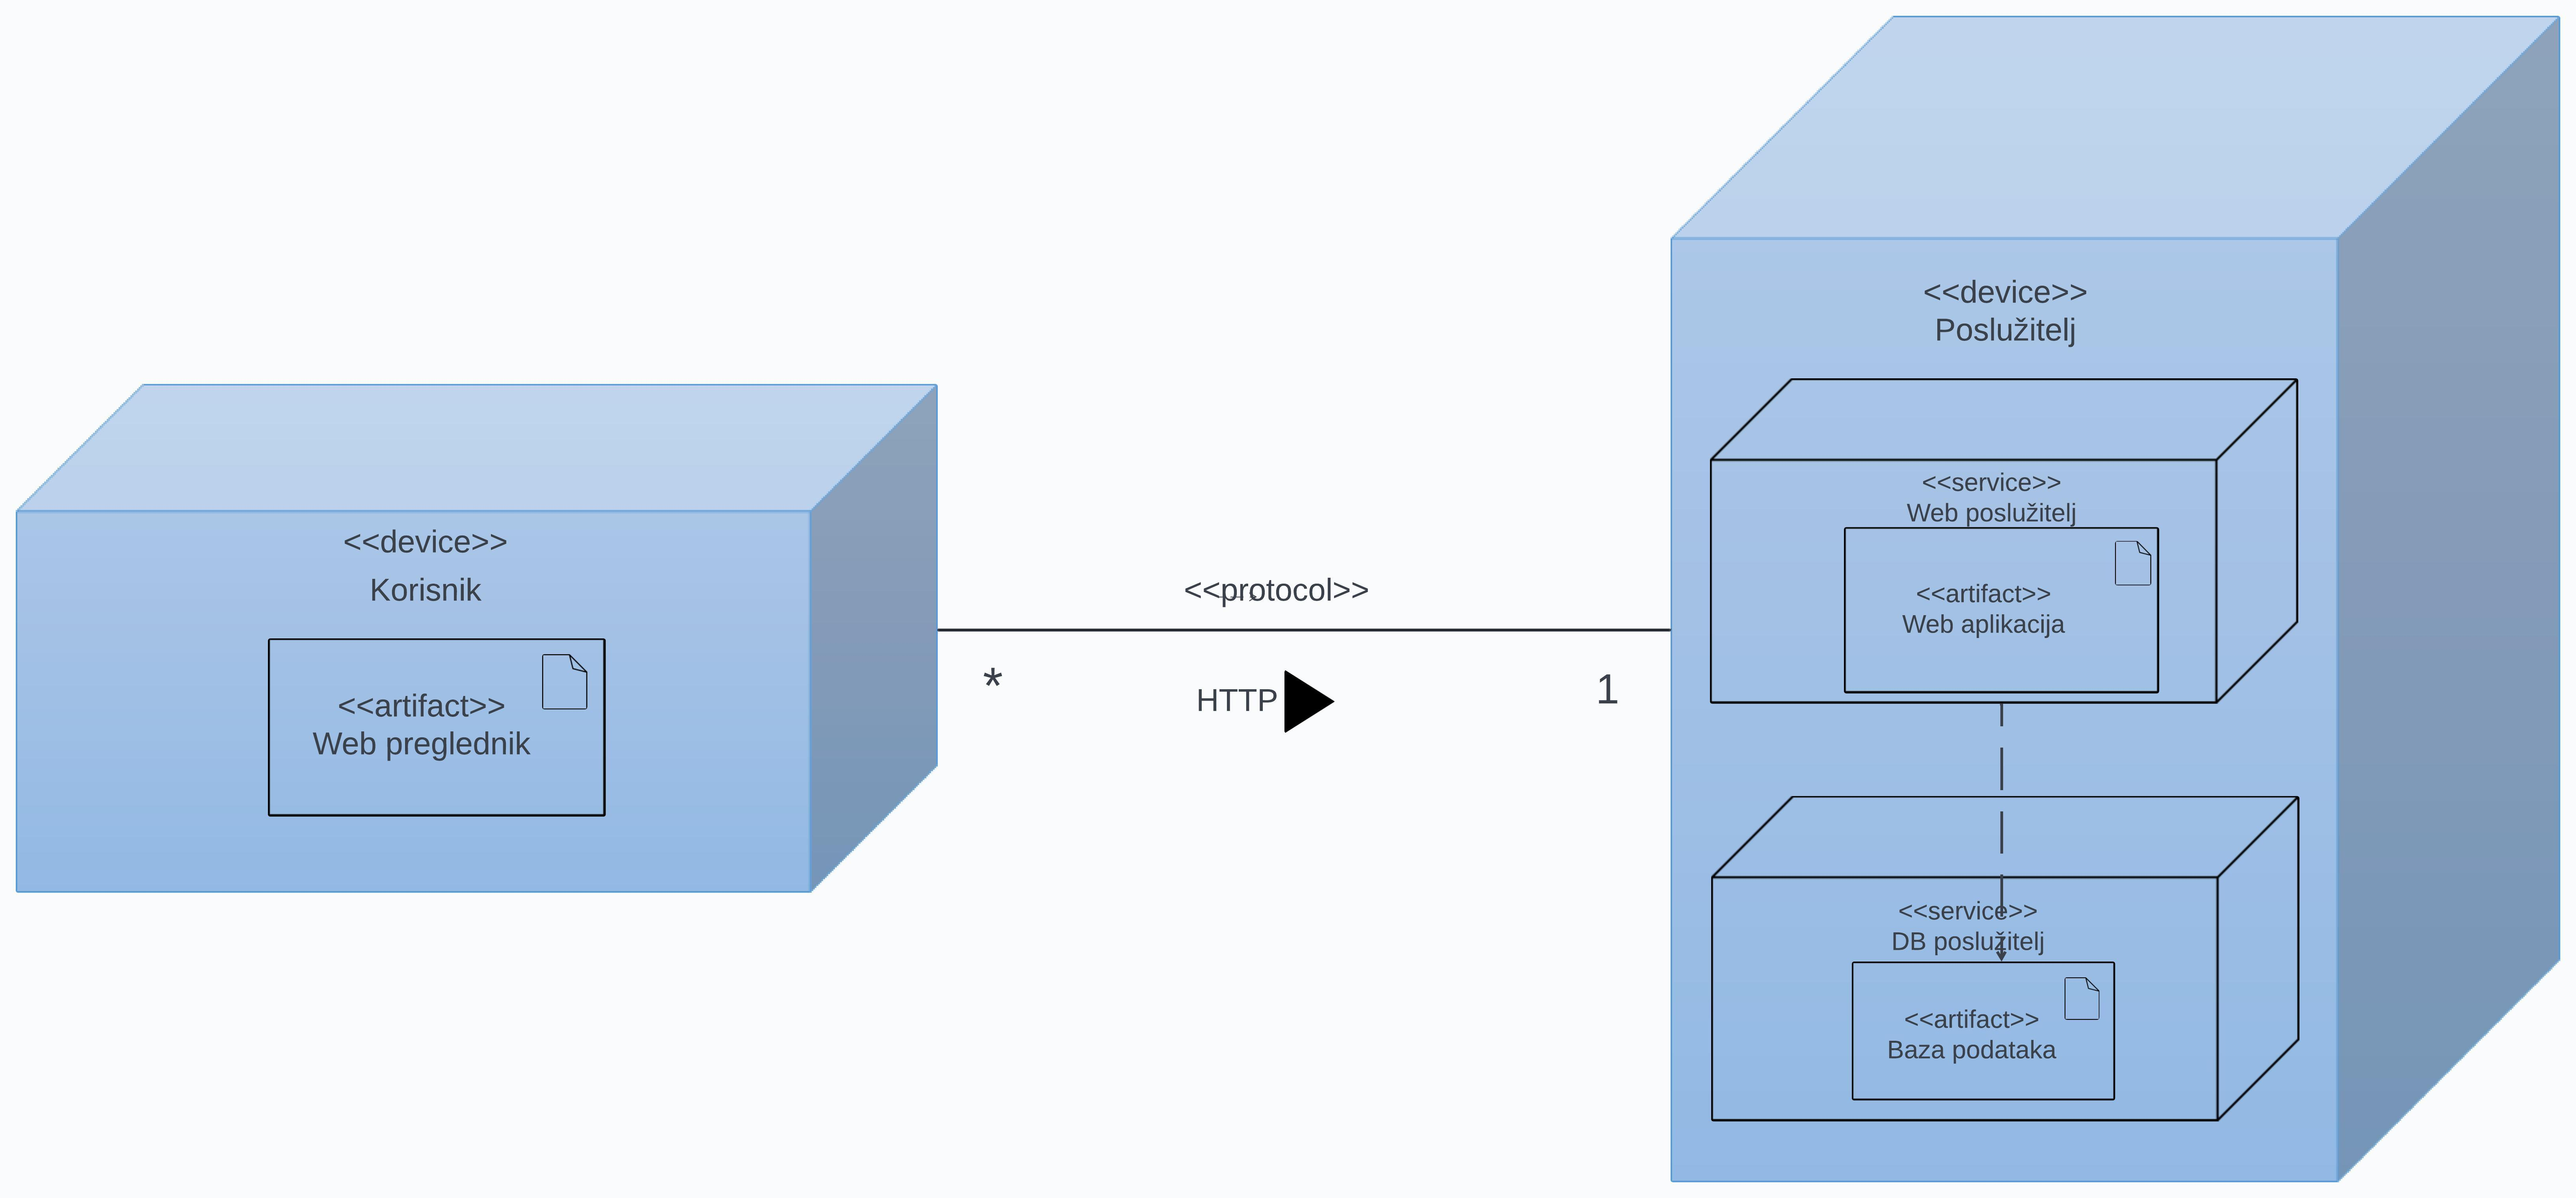
\includegraphics[scale=0.15]{dijagrami/Layout Diagram.jpeg}
			         \centering
			         \caption{Specifikacijski dijagram razmještaja}
			         \label{fig:LayoutDiagram}
		    \end{figure}
			
			\eject 
		
		\section{Upute za puštanje u pogon}
		
			Aplikacija je uspješno implementirana i dostupna na platformi Netlify. Za poslužitelj backend-a koristi se alat Render. Kako bi iskoristili sve korisne značajke koje Render pruža, potrebno je stvoriti instance baze podataka, poslužitelja za backend, te poslužitelja za frontend aplikacije. Prvi korak je kreiranje PostgreSQL baze podataka.
			
			\begin{figure}[H]
				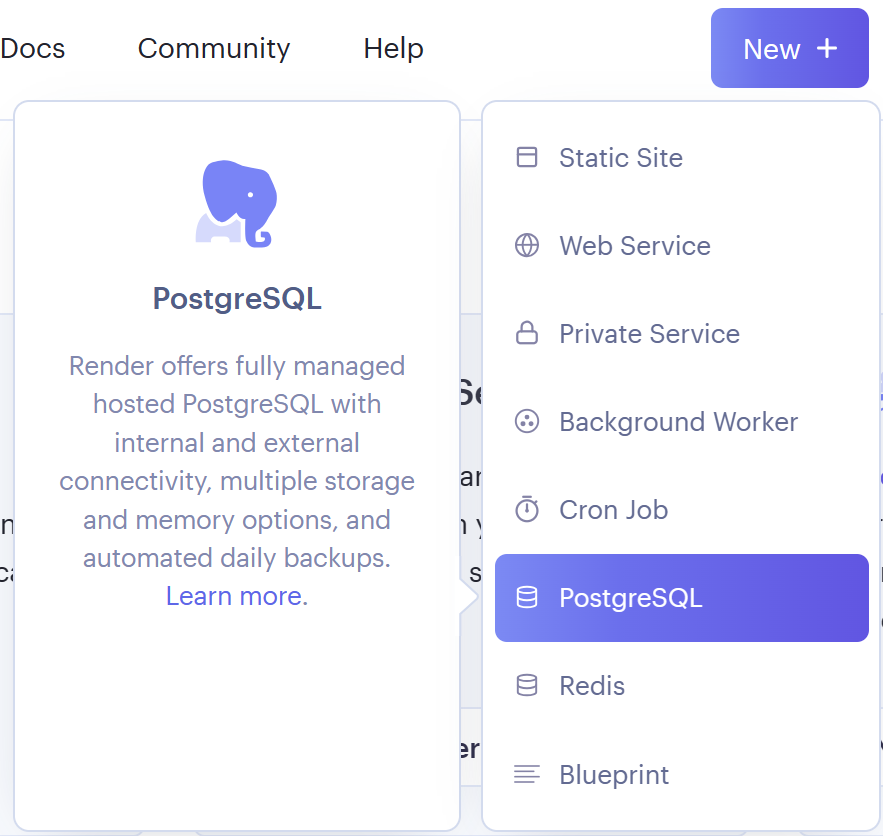
\includegraphics[scale=0.15]{dijagrami/PostgresSQL.jpeg}
				\centering
				\caption{Izbornik za stvaranje nove baze podataka}
				\label{fig:PostgresSQL}
			\end{figure}
			
			\eject 
			
			Potrebno je upisati ime baze, odabrati regiju poslužitelja instance i označiti tip instance koji će se koristiti.
			
			\begin{figure}[H]
				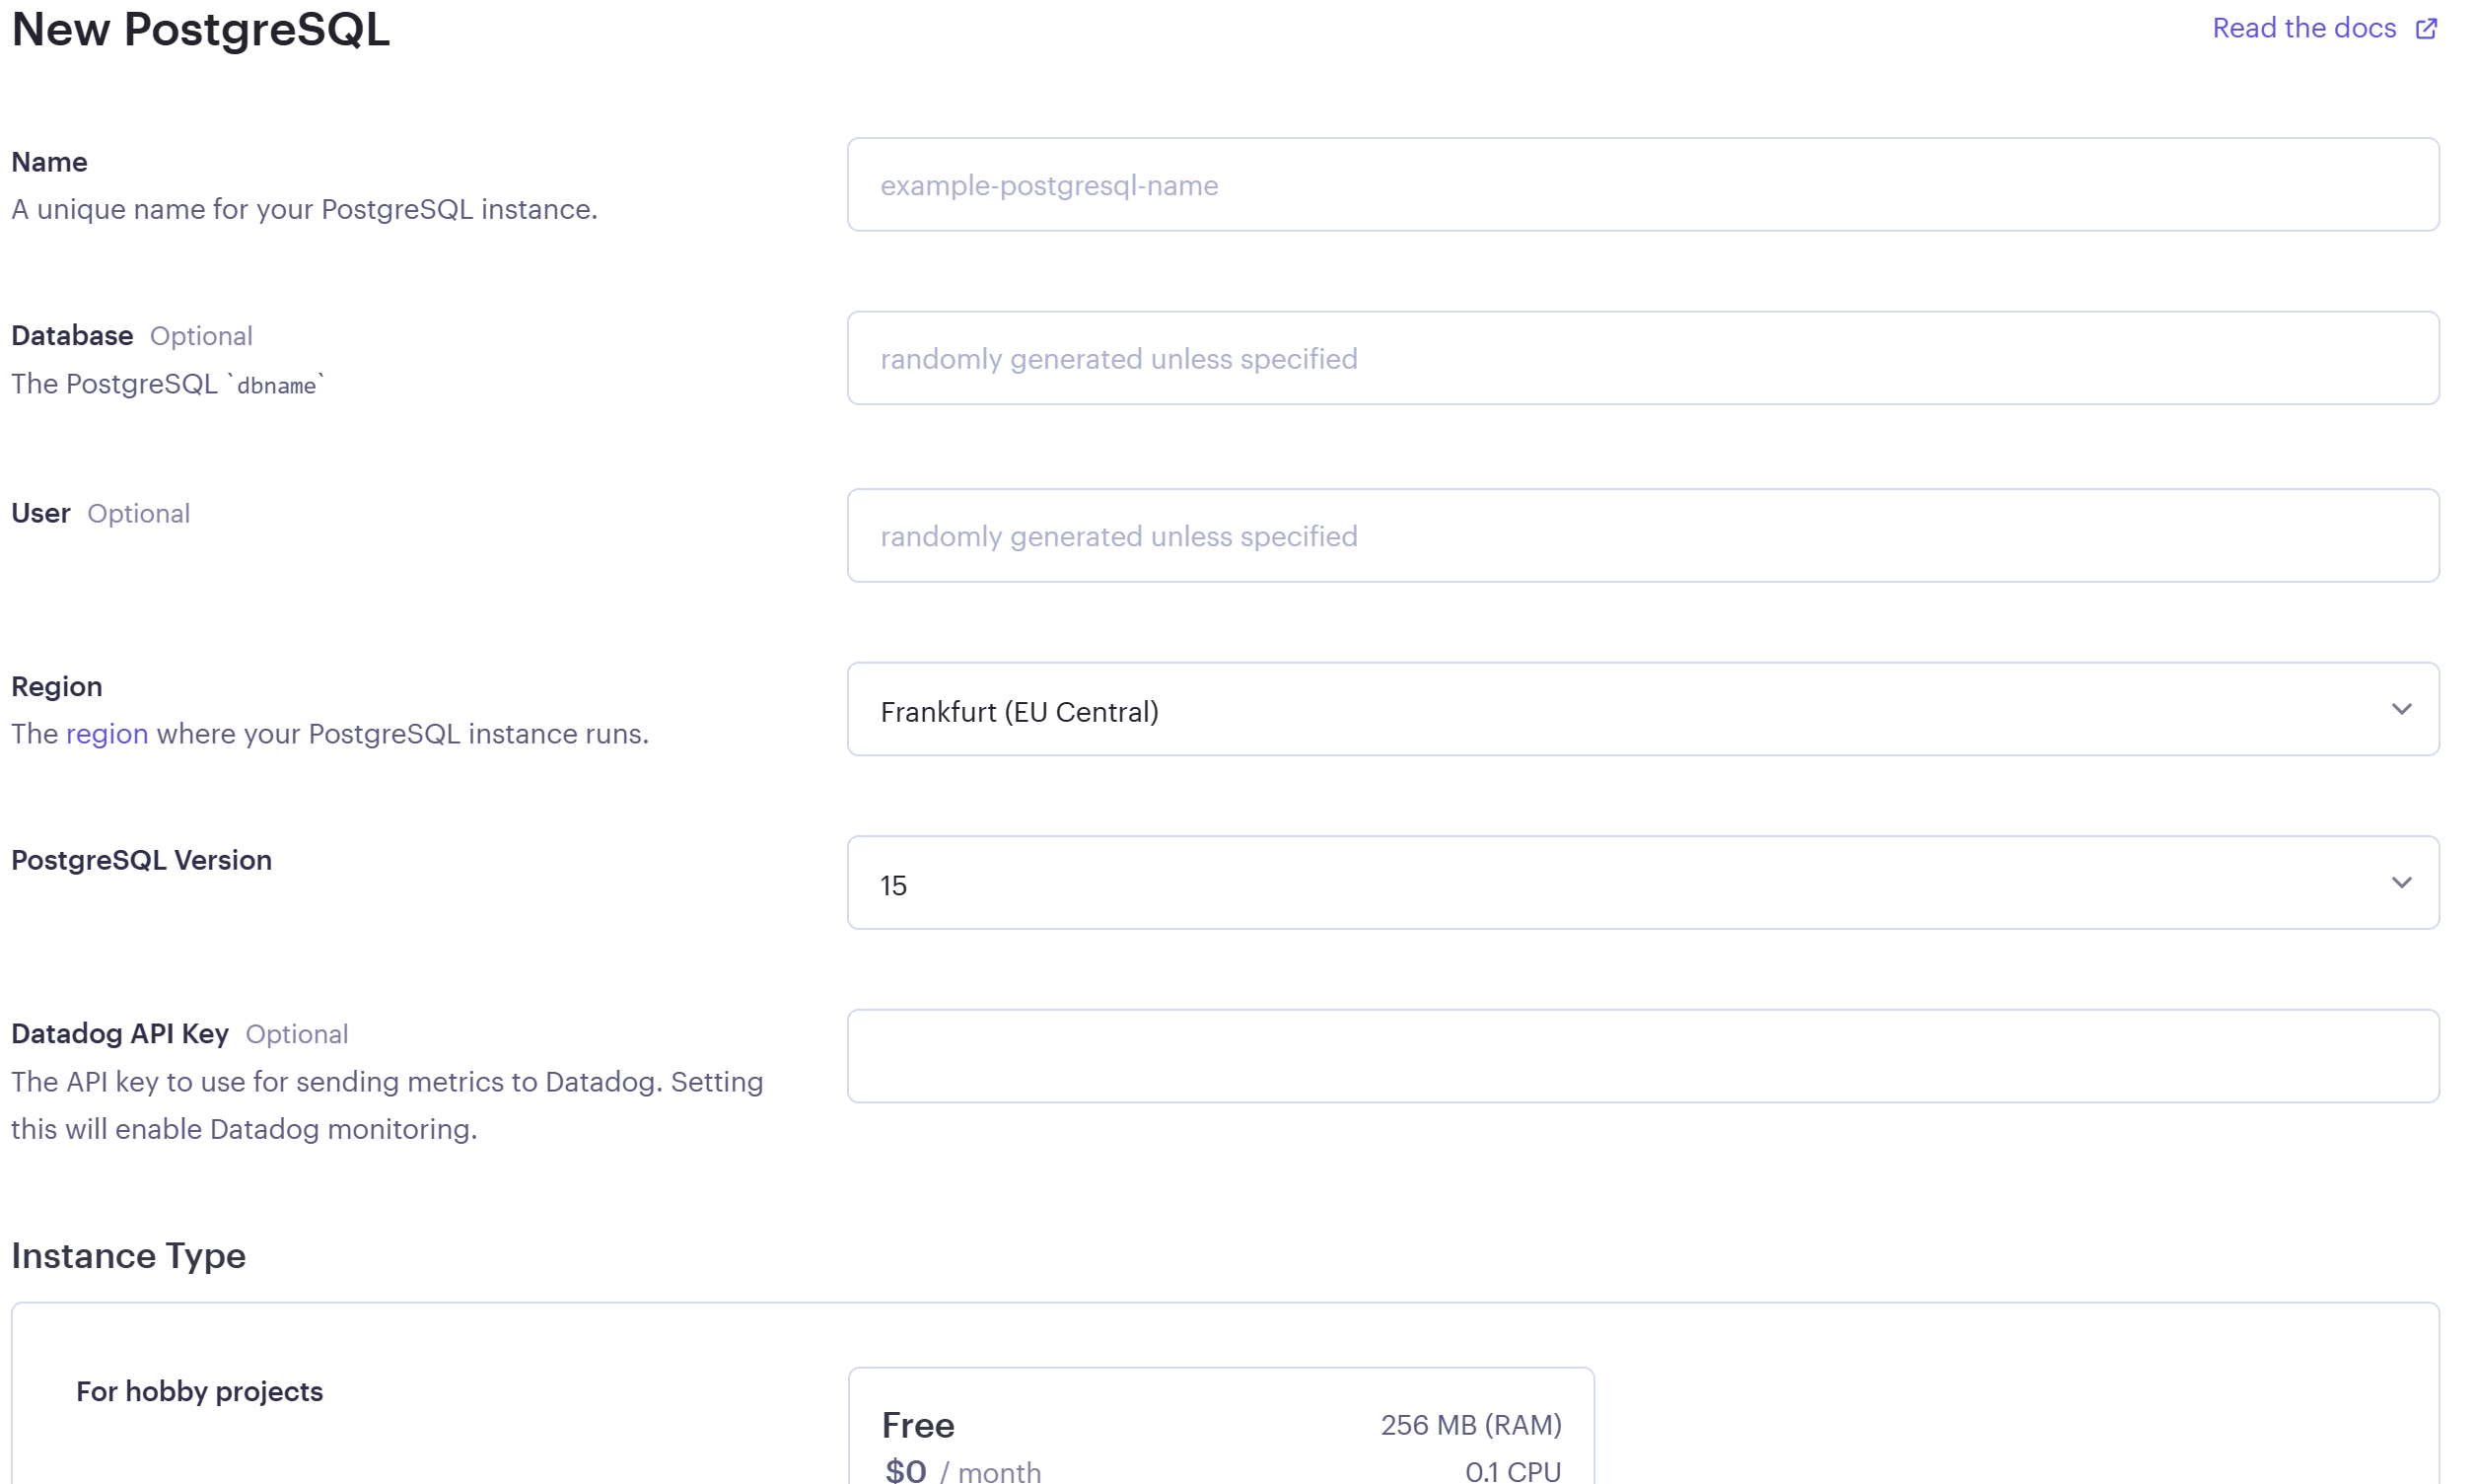
\includegraphics[scale=0.15]{dijagrami/stvaranje-baze.jpeg}
				\centering
				\caption{Stvaranje nove baze podataka}
				\label{fig:stvaranje-baze}
			\end{figure}
			
			\eject
			
			Nakon ovih koraka treba pokrenuti stvaranje pritiskom na tipku ”Create”.
			Pokazuje se prozor u kojemu su navedeni osnovni podaci o bazi kao ime, verzija, regija, prostor za pohranu, API ključ, itd.
			Kad je baza uspješno kreirana, potrebno je uzeti podatke koje treba dati backendu aplikacije. Ti podatci se nalaze u poljima \textit{Hostname}, \textit{Port}, \textit{Database}, \textit{Username}, \textit{Password} i \textit{External Database URL}.
			
			\pagebreak
			
			Backend je implementiran na Render platformi, koristeći Docker slike koje se automatski generiraju i implementiraju prilikom svakog push-a na master granu. Proces implementacije upravlja se pomoću GitHub Actions radnog toka definiranog u datoteci \textit{build-test-deploy.yaml}, koji obuhvaća korake poput preuzimanja koda, postavljanja JDK 17, izgradnje, testiranja, kopiranja JAR datoteke i prijenosa artefakta. Docker slika se označava tijekom procesa izgradnje. 
			
			\begin{figure}[H]
				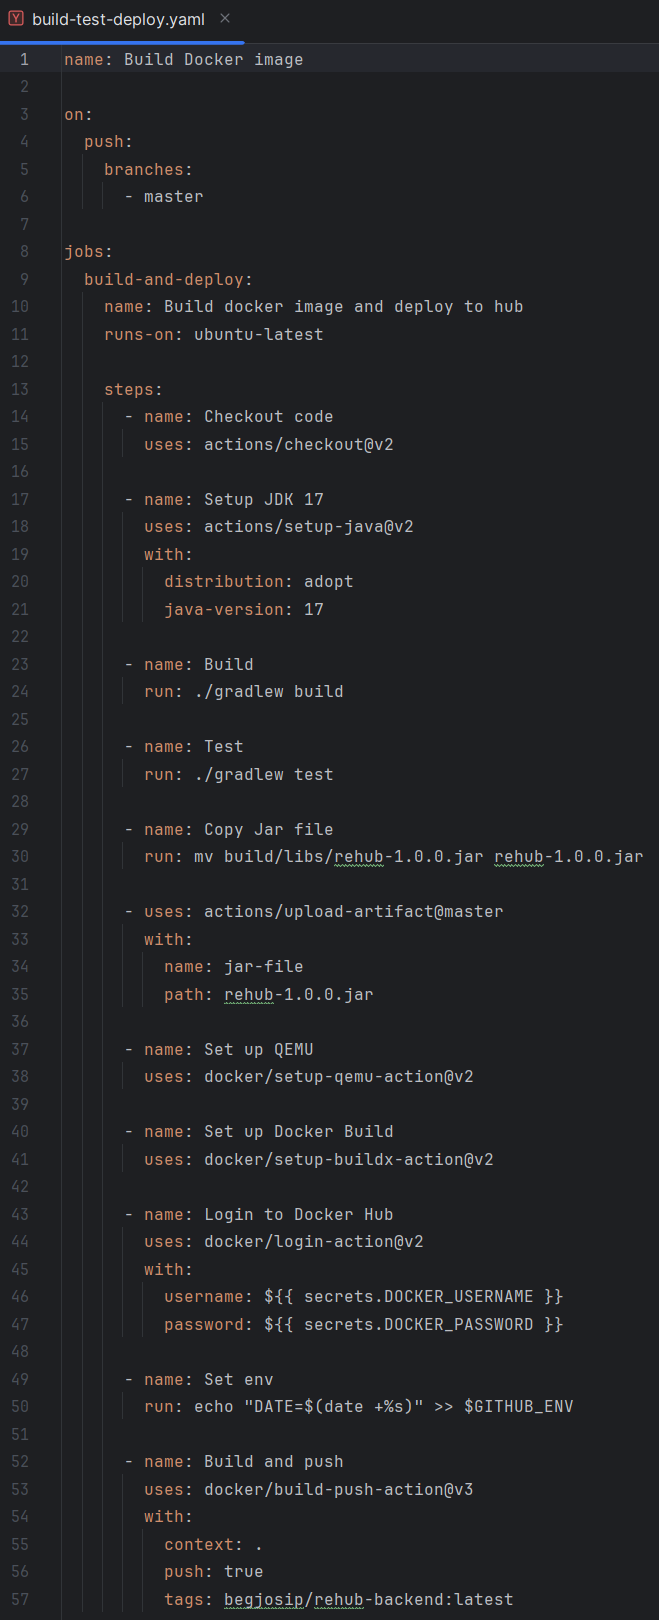
\includegraphics[scale=0.15]{dijagrami/built-test-deploy.jpeg}
				\centering
				\caption{Datoteka \textit{Datoteka build-test-deploy}}
				\label{fig:built-test-deploy}
			\end{figure}
			
			\eject
			
			Konfiguracija backend-a upravlja se putem datoteke \textit{application-prod.properties}, koja sadrži ključne parametre za konfiguraciju poslužitelja, prijenosa datoteka, podatkovnog izvora, e-pošte, ponovnog postavljanja lozinke, provjere korisnika, JPA i Flyway konfiguraciju te Jackson konfiguraciju. Svi ovi parametri su pažljivo prilagođeni kako bi podržali funkcionalnosti i integracije aplikacije, čime se osigurava glatki i učinkoviti razvojni i implementacijski proces backend-a.
			
			\begin{figure}[H]
				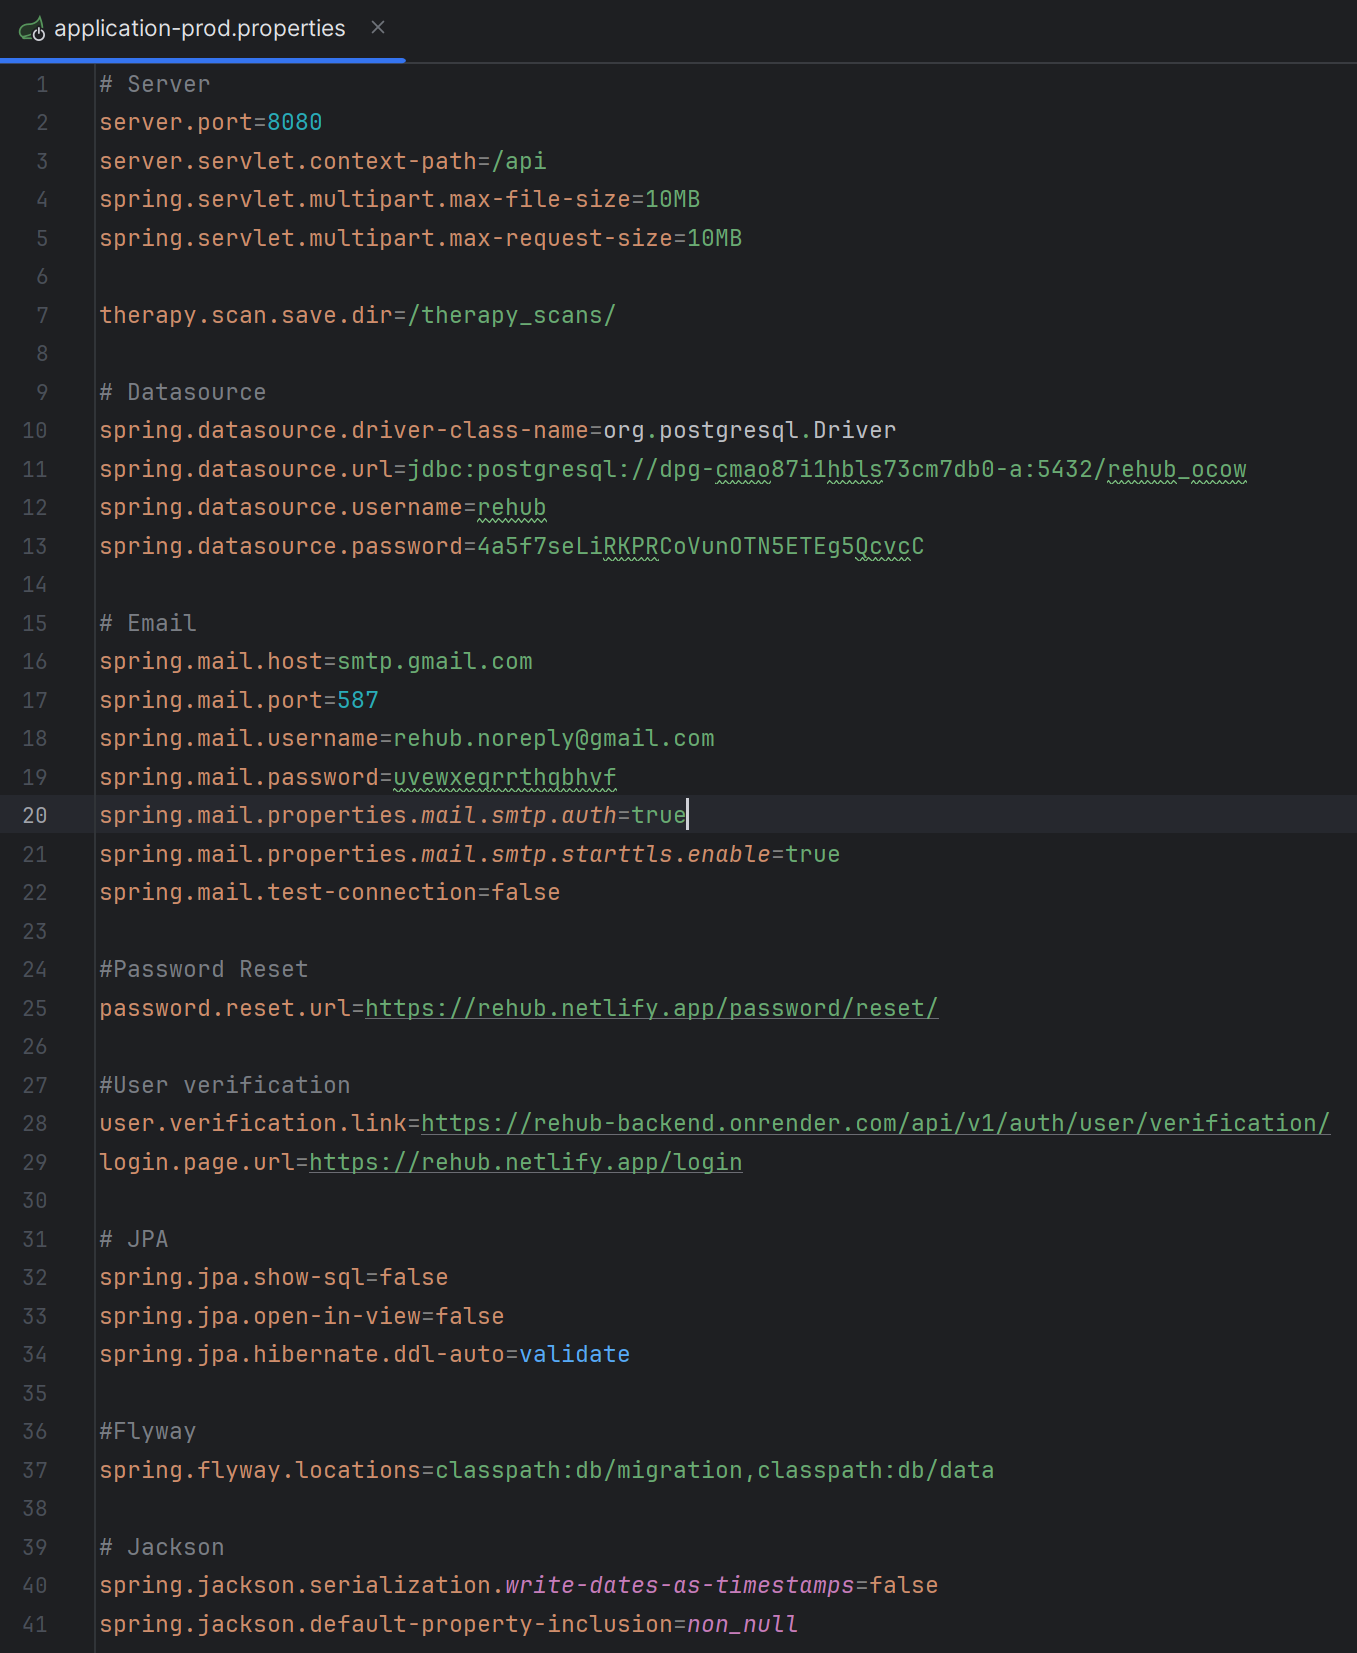
\includegraphics[scale=0.15]{dijagrami/app-prod.jpeg}
				\centering
				\caption{Datoteka \textit{application-prod.properties}}
				\label{fig:app-prod}
			\end{figure}
			
			\eject
			
			URL backend-a: https://rehub-backend.onrender.com/
			
			\pagebreak
			
			Frontend aplikacija je postavljena za automatski deploy na Netlify prilikom push-a na master granu. U datoteci \textit{build-deploy.yaml} specificiran je GitHub Actions radni tok za deploy na Netlify. 	
			
			\begin{figure}[H]
				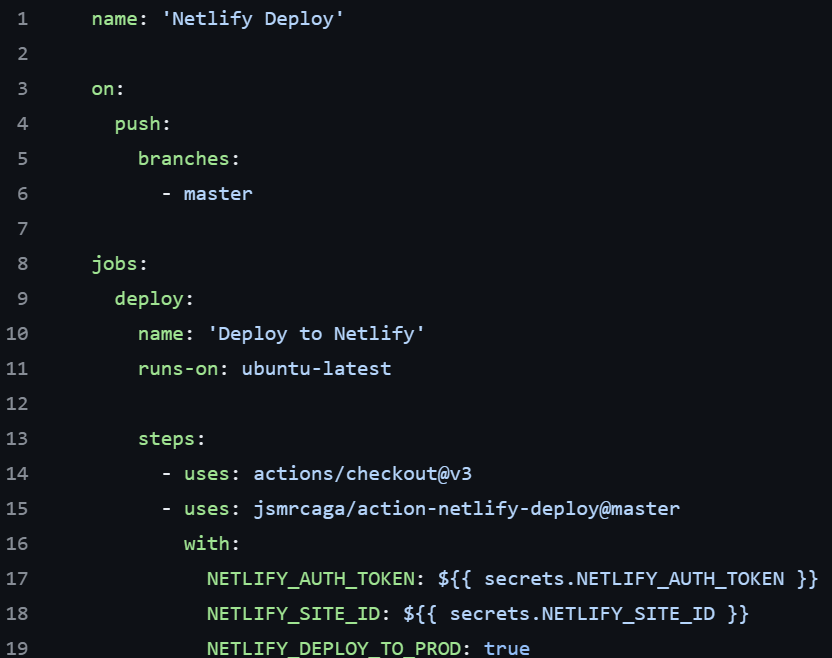
\includegraphics[scale=0.15]{dijagrami/bulid-and-deploy.jpeg}
				\centering
				\caption{Datoteka \textit{build-and-deploy.yaml}}
				\label{fig:build-and-deploy}
			\end{figure}
			
			\eject
			
			U Netlify konzoli, u postavkama projekta, konfigurirajte \textit{build} opcije.
			
			\begin{figure}[H]
				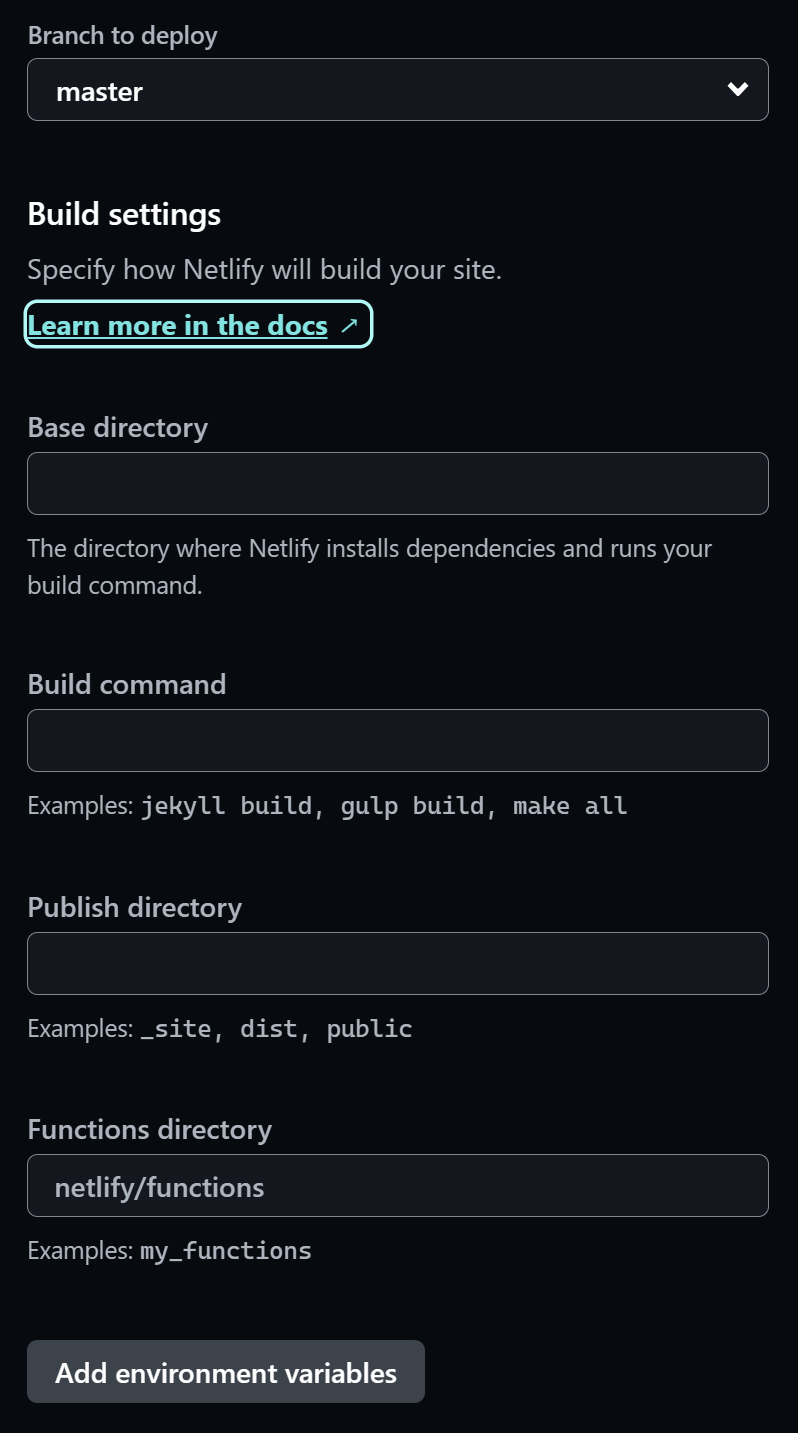
\includegraphics[scale=0.15]{dijagrami/netlify-conf.jpeg}
				\centering
				\caption{Postavljanje konfiguracije}}
				\label{fig:netlify-conf}
			\end{figure}
			
			\textit{Base Directory}: Postavite na direktorij u kojem se nalazi package.json.
			\textit{Build Command}: Postavite na naredbu koja pokreće izgradnju projekta, u ovom slučaju npm run build.
			\textit{Publish Directory}: Odredite direktorij koji sadrži izgrađene artefakte, u ovom slučaju build.
			
			\eject
			
			Aplikacija je puštena u pogon i spremna za uporabu. Pristupa se preko adrese koja je navedena za instancu frontenda.
			https://rehub.netlify.app
			
			\eject
			
			